% Chapter 2

\chapter{Theoretical Background} % Main chapter title

\label{Chapter2} % For referencing the chapter elsewhere, use \ref{Chapter2}

%----------------------------------------------------------------------------------------

\section{Satellite Altimetry observations}

Radar altimeter is a nadir looking microwave instrument. After its pulses are emitted, atmospheric corrections and an accurate determination of earth's orbit are applied, before information such as the the travel time of the return pulse and the shape of its waveform, provide us with the capability to  derive geophysical parameters. For this study, significant wave height and the wind speed at the surface of the ocean after being adjusted to 10 meters height, assuming neutral stability of the atmospheric boundary layer, will be used.

\begin{figure}[th]
\centering
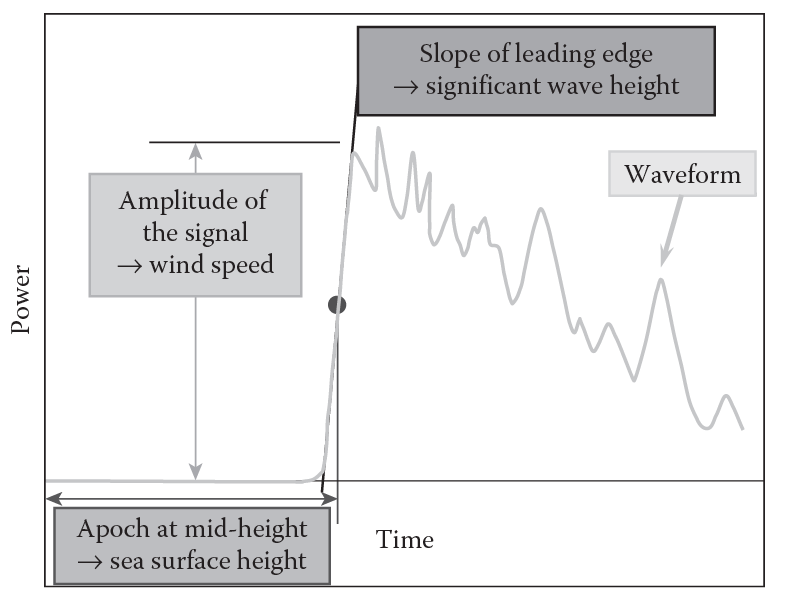
\includegraphics[width=\linewidth]{Figures/Chapter2/altimetry_principle.png}
%\decoRule
\caption{Significant wave height and wind speed from the radar altimeter waveform}
\label{fig:altimetry_principle}
\end{figure}

The wind speed can be measured because the strength of the backscatter signal is inversely proportional to the Mean Square Slope (MSS) of the sea surface. 

%----------------------------------------------------------------------------------------

